\chapter{研究内容}
\label{chap:contents}

本章では、本研究の内容を説明する。

\section{システム概要}

本システムの目的はユーザが必要とする複数の情報を提供することで、ユーザが効率良く価値の高い情報を得られるようにすることである。

以下にシステムの構成を示す。

\begin{table}[htbp]
  \caption{システム構成}
  \label{tb:files}
  \begin{center}\begin{tabular}{|c|p{12cm}|}
    \hline
    システム&概要\\\hline\hline
    {\tt Linda}\cite{linda}&データ元。データストリームからデータを取得する。\\\hline
    {\tt サーバ}&Androidクライアントからのリクエストがに応じLindaからデータを取得しAndroidクライアントに送信する。外部から取得したデータをLindaに書き込む。\\\hline
    {\tt WEBクライアント}&Androidクライアントに送信する情報を選択する為のビューを提供する。\\\hline
    {\tt Androidクライアント}&サーバにデータを要求し、ユーザに情報を表示する。\\\hline
    {\tt データベース}&サーバのデータを保存している。\\\hline
  \end{tabular}\end{center}
\end{table}

データをクラウド上で共有するためのフレームワークであるLindaを利用した。Lindaを利用することによって並列処理で同時に多くのクライアントを処理できる。

サーバは各種APIなどを用いてユーザが必要とする情報を取得しLindaへと書き込み、Androidクライアントからのリクエストに応じてLindaからデータを取得しJSON形式でレスポンスを返す。
Androidクライアントはユーザの操作に応じてサーバにリクエストを送り、サーバから返されたJSONをパースして表示する。

\subsection{データの取得と記録}
本システムでは三種類の方法でデータを取得している。

まず一つ目として既存のAPIを用いて取得する方法である。天気予報や株価の情報など比較的ポピュラーな情報であれば既にAPIが存在するので、それらを用いて定期的にサーバがデータを取得しLindaへ書き込む。(図\ref{fig:weather_widget})の例ではYahoo!の提供するAPIであるYQL\footnote{https://developer.yahoo.com/yql/}を用いて取得した天気予報をAndroid Widgetとして表示している。

\begin{figure}[htbp]
  \begin{minipage}{\hsize}
    \begin{center}
      \fbox{\includegraphics[width=100mm]{image/weather_widget.eps}}
    \end{center}
    \caption{天気予報をAndoid Widgetとして表示}
    \label{fig:weather_widget}
  \end{minipage}
\end{figure}

二つ目はAPIが存在しないWebページ上の情報である。例として自分の利用する公共交通機関の運行情報や特定の商品の在庫情報などである。これらのデータはKimono\footnote{https://www.kimonolabs.com/\\指定したWebページをスクレイピングし、API化するサービス。}というスクレイピングツールを用いて取得したい部分に対応するAPIを作成しデータを取得する。(図\ref{fig:odakyu_widget})の例では小田急電鉄のWebページ\footnote{http://www.odakyu.jp/cgi-bin/user/emg/emergency\_bbs.pl}(図\ref{fig:odakyu_page})にて公開されている列車の運行情報をKimonoを用いてAPI化して取得し、Android Widgetとして表示している。

\begin{figure}[htbp]
  \begin{minipage}{\hsize}
    \begin{center}
      \fbox{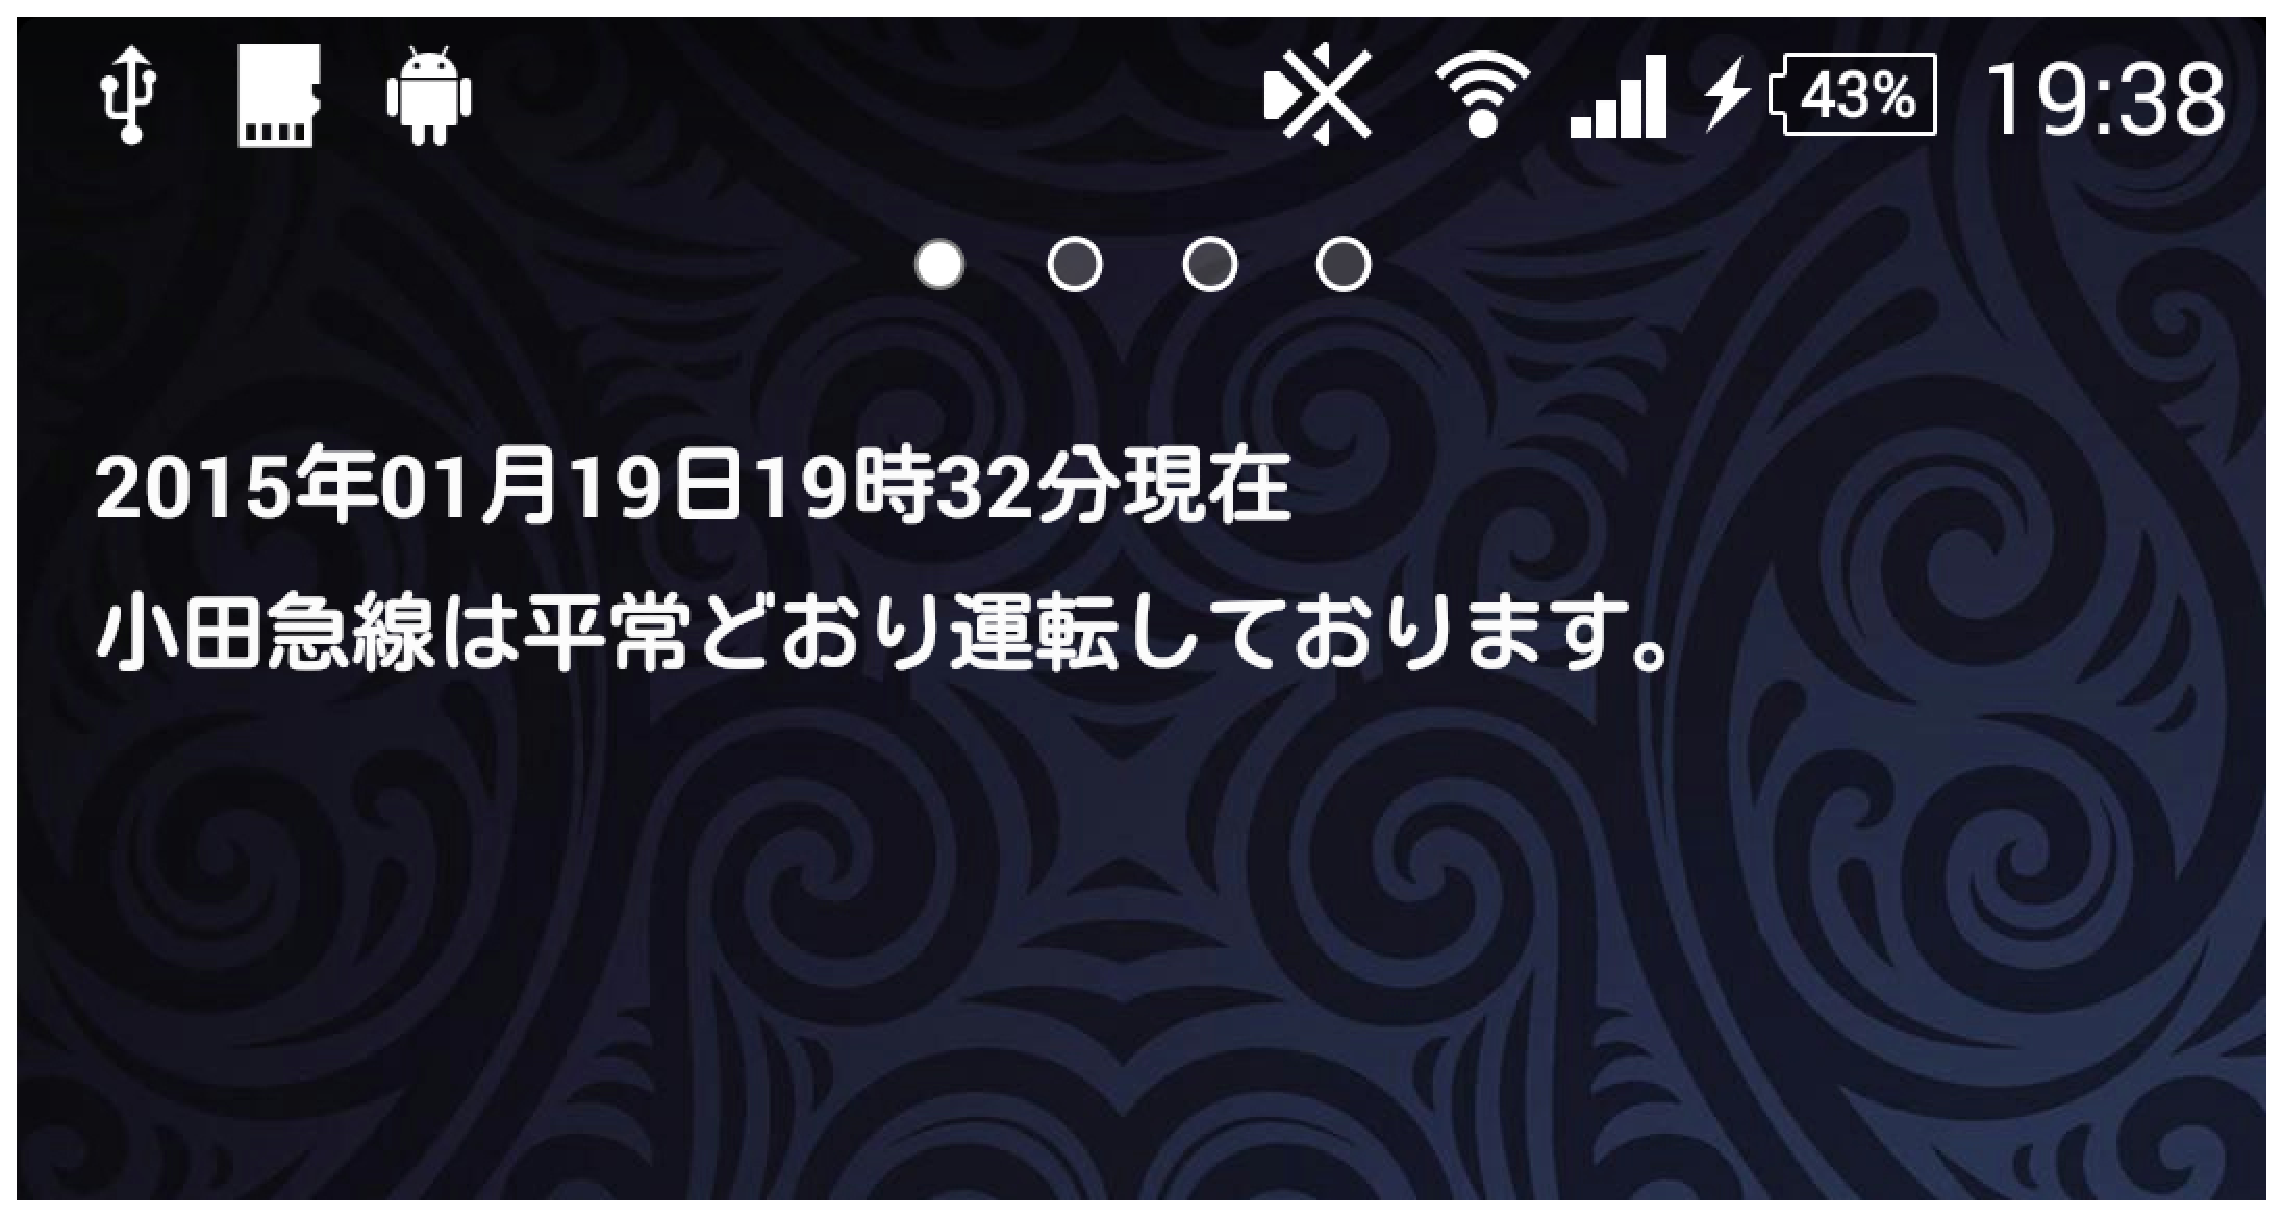
\includegraphics[width=100mm]{image/odakyu_widget.eps}}
    \end{center}
    \caption{小田急電鉄の運行情報を表示}
    \label{fig:odakyu_widget}
  \end{minipage}
\end{figure}

\begin{figure}[htbp]
  \begin{minipage}{\hsize}
    \begin{center}
      \fbox{
\includegraphics[width=100mm]{image/odakyu.eps}}
    \end{center}
    \caption{小田急電鉄の運行情報を公開しているWebページ}
    \label{fig:odakyu_page}
  \end{minipage}
\end{figure}

三つ目はセンシングデータである。自室などに設置した各種センサーからのデータに関してはセンシングする機器から直接Lindaに書き込むか、もしくはセンシングする機器からサーバ経由でLindaに書き込む。(図\ref{fig:arduino_sensor})はArduinoと明るさセンサー、温度センサーを用いてLindaにそれぞれの値を書き込こむ為の機構である。(図\ref{fig:sensor_widget})ではこの機構を用いて取得したデータを表示している。

\begin{figure}[htbp]
  \begin{minipage}{\hsize}
    \begin{center}
      \fbox{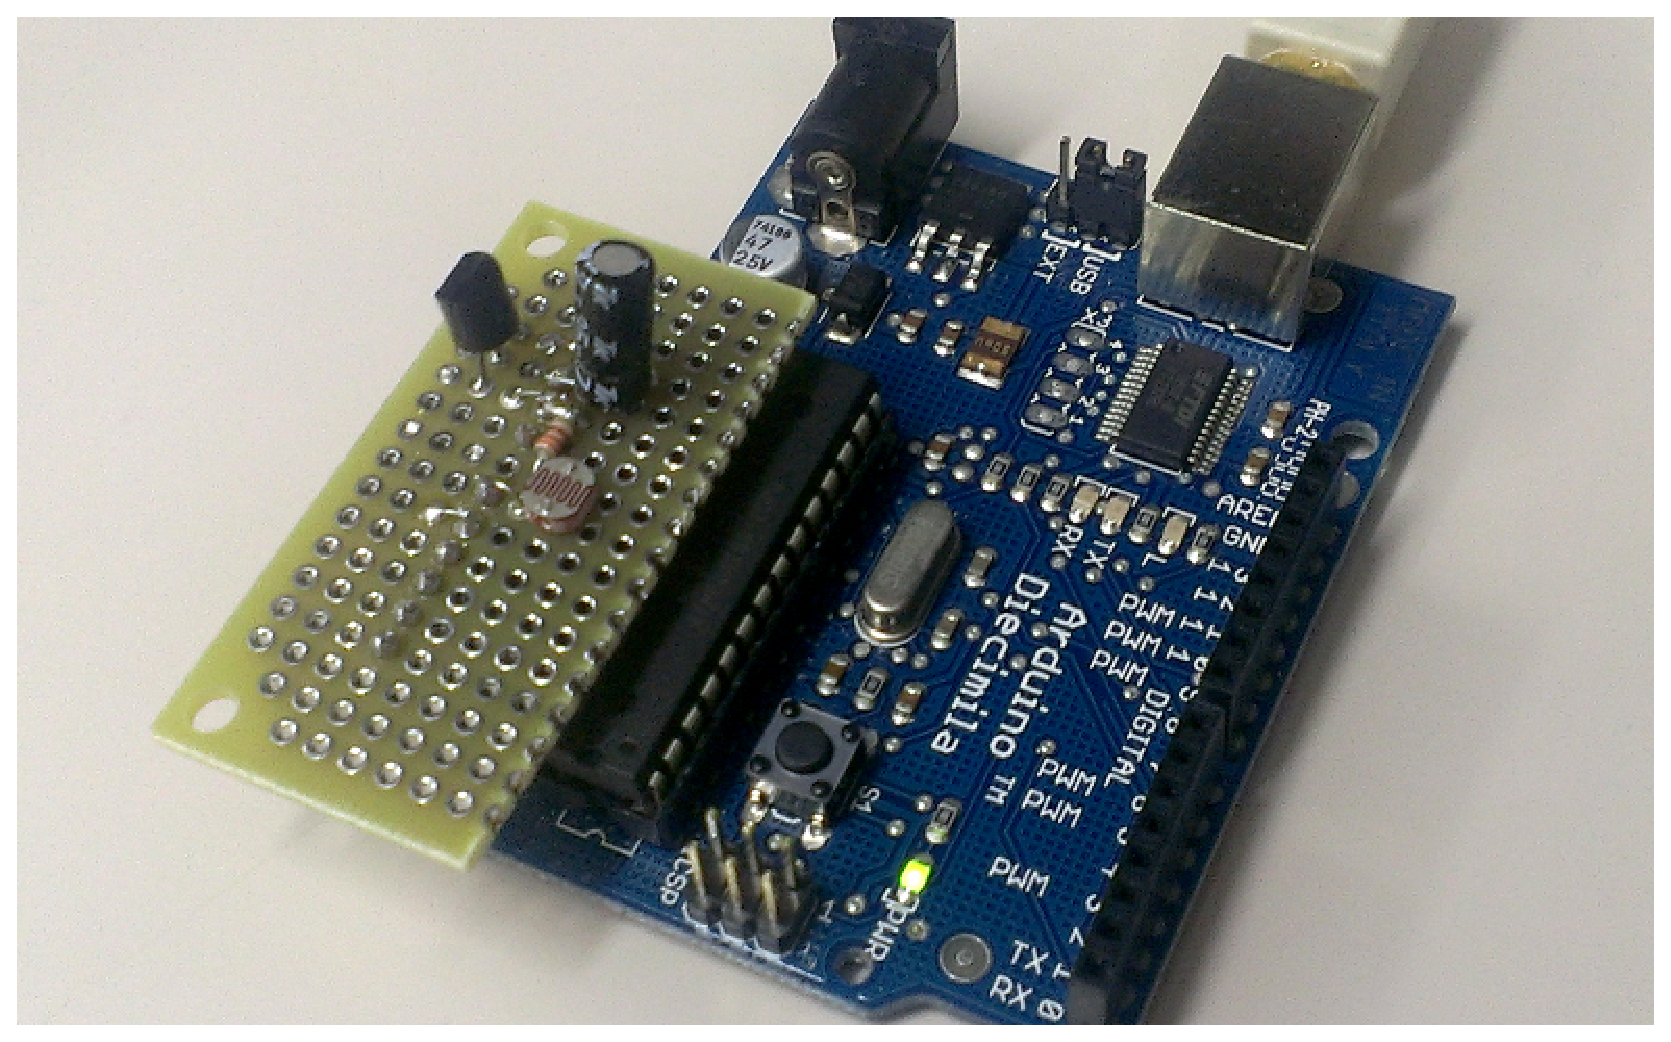
\includegraphics[width=100mm]{image/arduino_sensor.eps}}
    \end{center}
    \caption{明るさと温度を取得するセンサーとArduino}
    \label{fig:arduino_sensor}
  \end{minipage}
\end{figure}

\begin{figure}[htbp]
  \begin{minipage}{\hsize}
    \begin{center}
      \fbox{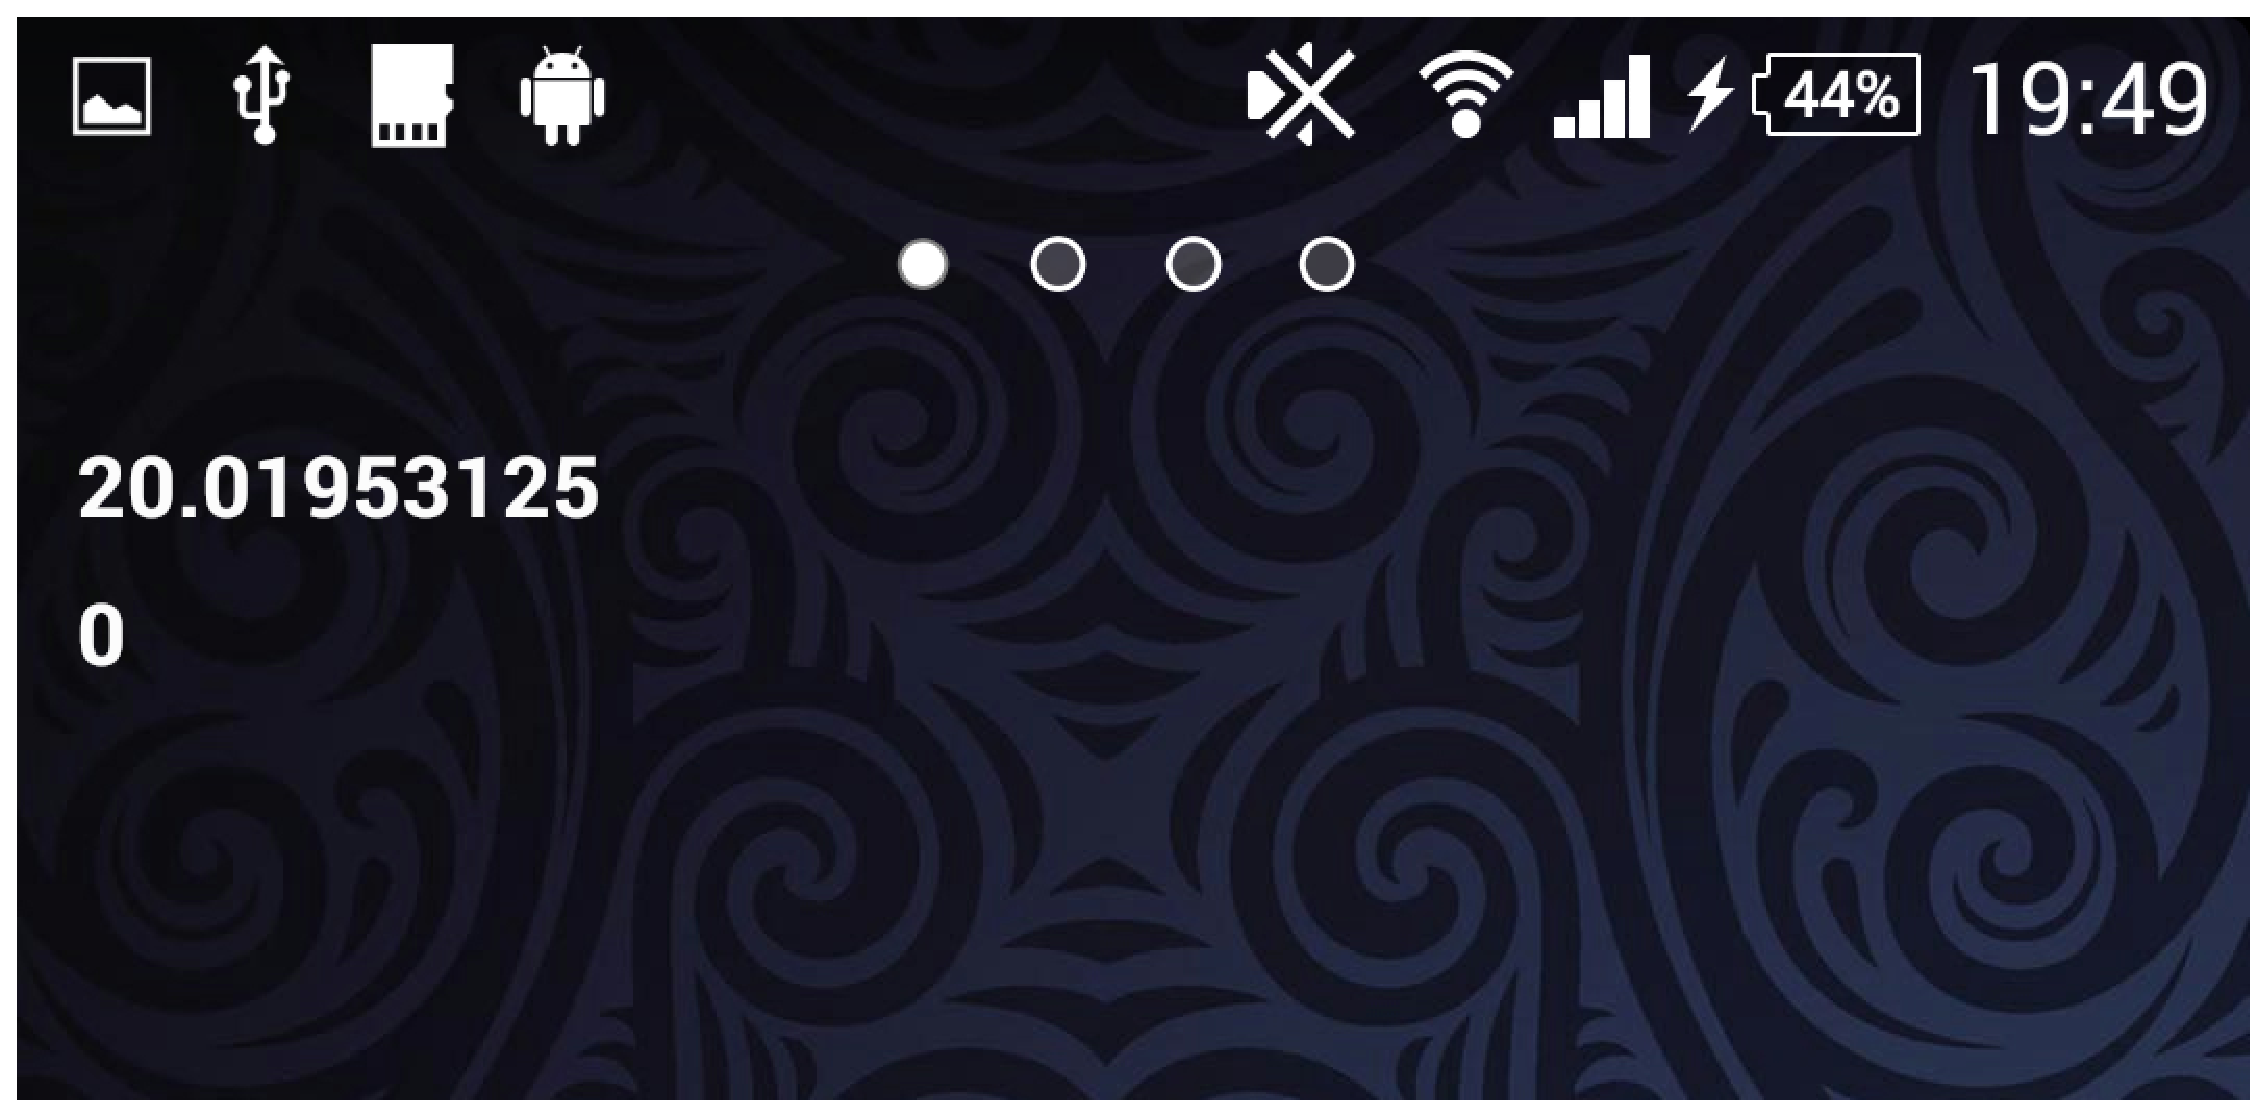
\includegraphics[width=100mm]{image/sensor_widget.eps}}
    \end{center}
    \caption{センサーデータをWidgetとして表示}
    \label{fig:sensor_widget}
  \end{minipage}
\end{figure}

\subsection{ユーザが受け取るデータの選択}

ユーザは受け取りたい情報をWebページ上から指定する。Lindaサーバに存在するデータの中から受け取りたい情報に対応したTupleTypeとTupleNameのペアを指定する。(図\ref{fig:select})このペアはデータベースに保存され、JSONを生成する際に参照される。

\begin{figure}[htbp]
  \begin{minipage}{\hsize}
    \begin{center}
      \fbox{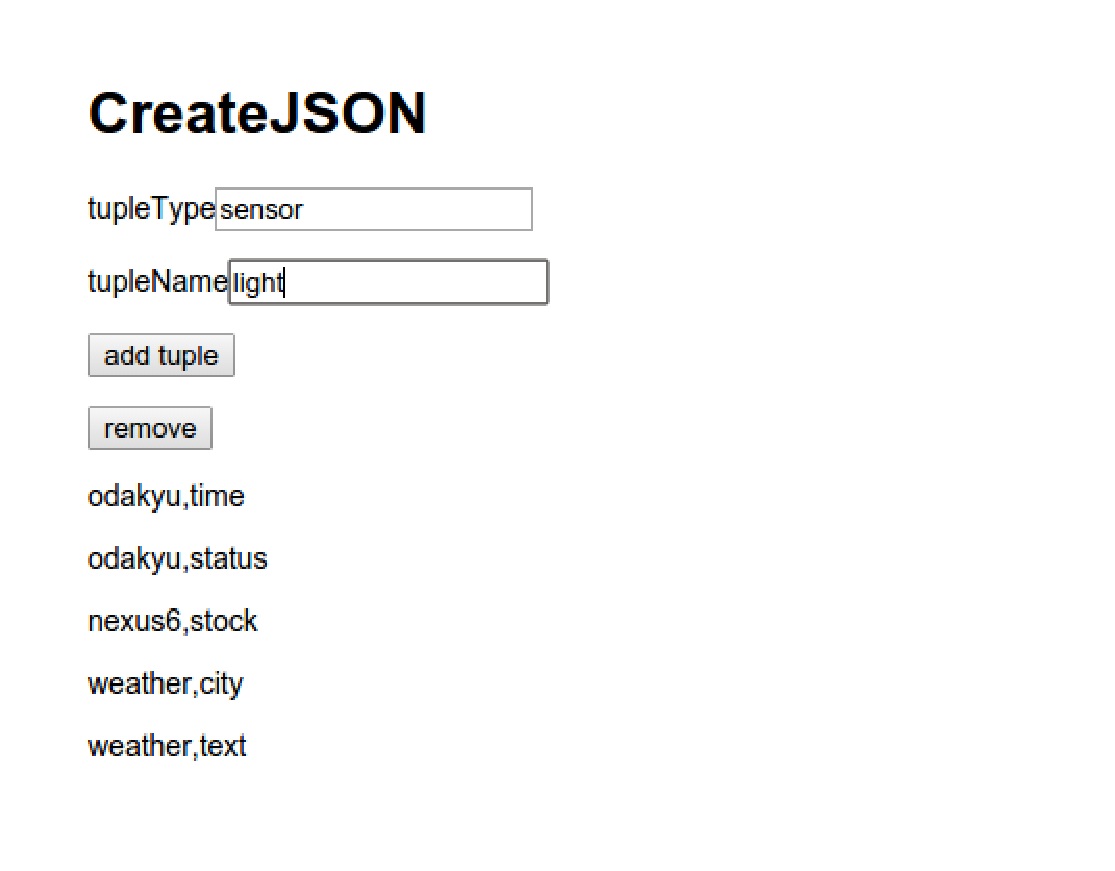
\includegraphics[width=100mm]{image/select.eps}}
    \end{center}
    \caption{Androidクライアントに送信するデータの選択画面}
    \label{fig:select}
  \end{minipage}
\end{figure}

\subsection{ユーザへの情報の提供}
ユーザが選択した情報はサーバによって取得されJSON形式でAndroid端末へと送られる。(図\ref{fig:JSON})Androidは受け取ったJSONをパースしAndroid Widgetとして表示する。(図\ref{fig:widget})

サーバへのリクエストは15分間隔のAndroid Widgetの自動更新の際と、ユーザがAndroid Widgetをタップした際に実行される。

\begin{figure}[htbp]
  \begin{minipage}{\hsize}
    \begin{center}
      \begin{lstlisting}[basicstyle=\ttfamily\footnotesize, frame=single]

      {
          "info": [
              {
                  "0": "2015年01月16日14時43分現在",
                  "1": "小田急線は平常どおり運転しております。",
                  "2": "We are out of inventory. Please check back soon.",
                  "3": "Fujisawa-shi",
                  "4": "Mostly Cloudy"
              }
          ]
      }

      \end{lstlisting}
    \end{center}
    \caption{サーバから送られるJSONの例}
    \label{fig:JSON}
  \end{minipage}
\end{figure}

\begin{figure}[htbp]
  \begin{minipage}{\hsize}
    \begin{center}
      \fbox{\includegraphics[width=100mm]{image/widget_single.eps}}
    \end{center}
    \caption{Android Widgetとして表示する例}
    \label{fig:widget}
  \end{minipage}
\end{figure}

\nocite{*}
